Let 
	\begin{align}
	 \vec{A} = \myvec{1\\2} , \vec{B} = \myvec{3 \\ 6}
	\end{align}
The direction vector 
\begin{align}
\vec{m}&= \vec{B}-\vec{A}=\myvec{2\\4}
\\
\implies 
    \vec{n}&= \myvec{-4\\2}
\end{align}
and 
\begin{align}
    c = \vec{n}^\top \vec {A} = \myvec{-4&2} \myvec{1\\2}=0 
\end{align}
This is verified in Fig. \ref{aug/76/2/fig:1}.
\begin{figure}[!ht]
\centering
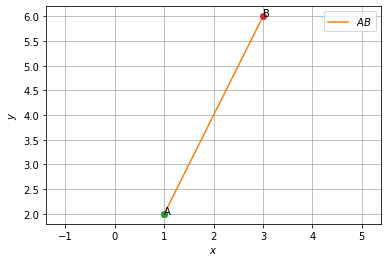
\includegraphics[width=\columnwidth]{solutions/aug/1/76/2/fig5.png}
\caption{LINE AB}
\label{aug/76/2/fig:1}
\end{figure}
